A seguir, são apresentadas perspectivas teóricas relevantes para o contexto do presente
trabalho.
\section{Sensoriamento remoto}
O sensoriamento remoto é uma disciplina fundamental em vários campos científicos e tecnológicos. Ele é definido  como:
\begin{quote}
"A arte ou ciência de dizer algo sobre um objeto sem tocá-lo." \parencite{fischer1976}
\end{quote}

Ao longo dos anos, o sensoriamento remoto tem evoluído significativamente, proporcionando uma variedade de aplicações em diversas áreas. Uma visão geral da evolução do sensoriamento remoto pode ser observada na Tabela \ref{tab:evolucao_sr}.

\begin{table}[!htb]
\caption{Evolução do sensoriamento remoto} \label{tab:evolucao_sr}
\begin{tabularx}{\textwidth}{|c|X|} \hline
\textbf{Ano} & \textbf{Evento} \\ \hline
1800         & Descoberta do infravermelho por Sir William Herschel \\ \hline
1839         & Início da prática da fotografia \\ \hline
1847         & Espectro infravermelho mostrado por A. H. L. Fizeau e J. B. L. Foucault para compartilhar propriedades com a luz visível \\ \hline
1850-1860    & Fotografia a partir de balões \\ \hline
1873         & Teoria da energia eletromagnética desenvolvida por James Clerk Maxwell \\ \hline
1909         & Fotografia a partir de aviões \\ \hline
1914-1918    & Primeira Guerra Mundial: reconhecimento aéreo \\ \hline
1920-1930    & Desenvolvimento e aplicações iniciais da fotografia aérea e fotogrametria \\ \hline
1929-1939    & Depressão econômica gera crises ambientais que levam a aplicações governamentais da fotografia aérea \\ \hline
1930-1940    & Desenvolvimento de radares na Alemanha, Estados Unidos e Reino Unido \\ \hline
1939-1945    & Aplicações da Segunda Guerra Mundial de porções não visíveis do espectro eletromagnético, treinamento de pessoas na aquisição e interpretação de fotografias aéreas \\ \hline
1950-1960    & Pesquisa e desenvolvimento militares \\ \hline
1956         & Pesquisa de Colwell sobre detecção de doenças de plantas com fotografia infravermelha \\ \hline
1960-1970    & Primeiro uso do termo sensoriamento remoto, satélite meteorológico TIROS, observações de sensoriamento remoto da Skylab do espaço \\ \hline
1972         & Lançamento do Landsat 1 \\ \hline
1970-1980    & Avanços rápidos no processamento digital de imagens \\ \hline
1980-1990    & Landsat 4: nova geração de sensores Landsat, satélite de observação terrestre SPOT da França \\ \hline
1980s        & Desenvolvimento de sensores hiperespectrais \\ \hline
1990s        & Sistemas globais de sensoriamento remoto, lidares \\ \hline
\end{tabularx}
\fonte{Adaptado de \textcite{campbell2011}.}
\end{table}

Uma das principais áreas de aplicação do sensoriamento remoto na atualidade é a agricultura. Estudos recentes, como o de \textcite{weiss2020}, destacam sua importância na adaptação e evolução das práticas agrícolas, fornecendo informações repetitivas sobre o estado das culturas ao longo da temporada, em diferentes escalas e para diferentes \textit{stakeholders}. 

Da mesma forma, pesquisas ressaltam suas vantagens na monitorização das culturas, estimativa de produtividade e tomada de decisão em diferentes estágios da produção agrícola \parencite{shanmugapriya2019, khanal2020}. Além disso, estudos evidenciam seu papel na obtenção de estatísticas agrícolas, contribuindo para a definição de unidades amostrais, estratificação e alocação de amostras \parencite{carfagna2005}.

\section{Telemetria}
A telemetria é um campo complementar ao sensoriamento remoto e é definida como:
\begin{quote}
"A indicação, registro ou integração de uma quantidade em um ponto remoto por meios eleitorais e de tradução métrica.  Grandezas de estados elétricos ou mecânicos estão normalmente envolvidas, embora existam outras aplicações diversas para telemedição." \parencite{telemetering1941}
\end{quote}

De acordo com \textcite{telemetry_systems2002}, ao longo das décadas, os sistemas de telemetria evoluiram gradativamente, impulsionada por avanços tecnológicos em eletrônica, comunicações e processamento de dados. Inicialmente, a telemetria era predominantemente utilizada em aplicações aeroespaciais e militares para monitorar o status e o desempenho de aeronaves e foguetes. 

No entanto, com o passar do tempo, sua aplicabilidade se expandiu para uma variedade de setores, incluindo medicina, indústria automotiva, energia e telecomunicações \parencite{Lizhuang_telemetry2021, Hassanien2020, Ding_telemetry2017}.

Para \textcite{Lizhuang_telemetry2021}, os avanços na miniaturização de sensores, aumento da capacidade de armazenamento de dados e melhorias nas técnicas de transmissão de dados tornaram possível a coleta e análise de uma quantidade cada vez maior de dados de telemetria. Além disso, \textcite{Ding_telemetry2017} afirmam que o desenvolvimento de algoritmos de análise de dados e inteligência artificial (IA) tem permitido uma compreensão mais profunda dos padrões e tendências nos dados telemétricos, levando a aprimoramentos em diversos processos e sistemas.

\section{Sistemas embarcados}
Há várias concepções propostas para sistemas embarcados, sendo a mais difundida definida como:

\begin{quote}
"Aquele que possui \textit{hardware} de computador com \textit{software} embutido como um de seus componentes mais importantes. É um sistema baseado em computador dedicado para uma ou várias aplicações. Pode ser um sistema independente ou parte de um sistema maior." \parencite{dutta2014comprehensive}
\end{quote}

Sua utilização abrange desde dispositivos simples, como controles remotos e eletrodomésticos, até sistemas complexos, como veículos autônomos e equipamentos médicos \parencite{lee2008cyber, kato2018autoware}. Eles desempenham um papel fundamental na automação de processos industriais, na monitoração e controle de dispositivos, na coleta e processamento de dados em tempo real, entre outras funções \parencite{dutta2014comprehensive}.

Segundo \textcite{lee2008cyber}, os microcontroladores são componentes essenciais dos sistemas embarcados. Estes desempenham um papel central na execução de tarefas específicas e no controle de dispositivos em uma variedade de aplicações. Eles são dispositivos de computação completos, contendo não apenas uma unidade central de processamento (CPU), mas também memória, periféricos de entrada e saída (E/S) e, muitas vezes, interfaces de comunicação \parencite{dutta2014comprehensive}. 
A Tabela \ref{tab:evolucao_microcontroladores} mostra alguns modelos de microcontroladores e suas finalidades, desde modelos mais antigos até os mais recentes.

\begin{table}[!htb]
\caption{Evolução dos microcontroladores} \label{tab:evolucao_microcontroladores}
\begin{tabularx}{\textwidth}{|c|c|X|} \hline
\textbf{Modelo} & \textbf{Ano de Lançamento} & \textbf{Finalidade} \\ \hline
Intel 8051 & 1977 & Controle de dispositivos básicos  \parencite{8051_usage} \\ \hline
PIC16F84A & 1993 & Automação residencial e controle de pequenos dispositivos \parencite{PIC16F84A_usage} \\ \hline
Arduino Uno & 2010 & Prototipagem rápida e educação em eletrônica \parencite{Arduino_usage} \\ \hline
STM32F4 & 2011 & Controle embarcado avançado e processamento de sinais \parencite{STM32F4_usage} \\ \hline
ESP32 & 2016 & Aplicações IoT avançadas e sistemas de monitoramento \parencite{ESP32_usage} \\ \hline
Raspberry Pi 4 & 2019 & Desenvolvimento de sistemas embarcados e IoT  \parencite{RaspberryPi4_usage} \\ \hline
\end{tabularx}
\fonte{Elaborado pelo autor, 2024.}
\end{table}

\section{Sistemas cyberfísicos}

Os sistemas cyberfísicos (CPSs) representam uma evolução dos sistemas embarcados. Eles são definidos como:

\begin{quote}
"Integrações de computação com processos físicos. Computadores embarcados e redes que monitoram e controlam os processos físicos, geralmente com loops de \textit{feedback} onde os processos físicos afetam as computações e vice-versa." \parencite{lee2008cyber}
\end{quote}

Recentemente, tem havido uma tendência crescente no uso de CPSs em aplicações práticas. Por exemplo, \textcite{ahmad2020smart} demonstraram um sistema de monitoramento inteligente de campo que utiliza abordagens para rastrear o comportamento e as atividades de roedores no campo. O sistema auxilia especialistas em controle de pragas e agricultores na aplicação mais eficiente de métodos de controle tradicionais.

Da mesma forma, \textcite{rad2015smart} propuseram um modelo de arquitetura de CPS para o monitoramento inteligente de culturas de batata na agricultura de precisão resultando na melhoria da produtividade. Além disso, \textcite{rijswijk2021digital} discutiram o papel dos sistemas socio-cyberfísicos (SCPSs) na transformação digital da agricultura e das áreas rurais. Eles destacaram a necessidade de compreender as relações entre os aspectos sociais e tecnológicos para uma aplicação bem-sucedida.

\section{ESP32}

O ESP32 é um microcontrolador de baixo custo desenvolvido pela Espressif Systems. De acordo com \textcite{ESP32_usage}, este componente é amplamente utilizado em projetos de IoT devido às suas capacidades de conexão integradas e poder de processamento.

Baseado em um processador \textit{dual-core} Tensilica Xtensa LX6, o ESP32 opera em frequências de até 240 MHz, apresentando uma arquitetura de 32 bits. Além disso, possui uma variedade de periféricos, incluindo GPIOs, UARTs, SPIs e I2Cs, conforme descrito na Tabela \ref{tab:esp32_perifericos}, o que o torna altamente versátil para uma ampla gama de aplicações \parencite{EspressifESP32}.

Uma das principais vantagens do ESP32, como destacado por \textcite{ESP32_usage}, é sua capacidade de conexão Wi-Fi e Bluetooth embutida, suportando os padrões 802.11 b/g/n Wi-Fi, Bluetooth 4.2 e Bluetooth Low Energy (BLE). Isso possibilita a comunicação sem fio em ambientes de IoT.

O ESP32 pode ser programado usando o Arduino IDE e o ESP-IDF (Espressif IoT Development Framework), ambos baseados em C/C++. Através dessas plataformas de desenvolvimento, os desenvolvedores podem acessar os recursos do ESP32 e criar uma variedade de aplicações, desde simples projetos de automação residencial até dispositivos complexos de monitoramento e controle \parencite{ferrandez2018precision, junior2022data, hsu2020creative}.

\begin{table}[!htb]
  \caption{Periféricos do microcontrolador ESP32} \label{tab:esp32_perifericos}
  \begin{tabularx}{\textwidth}{|c|X|X|} \hline
    \textbf{Abreviação} & \textbf{Nome} & \textbf{Função} \\ \hline
    GPIO & Entrada/saída de uso geral & Permite a comunicação de propósito geral com dispositivos externos através de sinais de entrada e saída digitais  \\ \hline
    UART & Receptor/transmissor assíncrono universal & Facilita a comunicação serial assíncrona entre o microcontrolador e outros dispositivos, como sensores e módulos de comunicação \\ \hline
    SPI & Interface periférica serial & Permite a comunicação serial síncrona de alta velocidade entre o microcontrolador e dispositivos periféricos, como sensores, displays e memórias \\ \hline
    I2C & Circuito Interintegrado & Oferece uma interface serial de dois fios para comunicação entre vários dispositivos \\ \hline
  \end{tabularx}
  \fonte{Adaptado de \textcite{EspressifESP32}.}
\end{table}

\section{Internet das coisas}
A Internet das Coisas (IoT) é um campo multidisciplinar que se desenvolveu ao longo do tempo, com contribuições de diversas áreas, incluindo computação, telecomunicações, eletrônica e engenharia (Figura \ref{figura:evolucao_iot}). Ela é definida como:

\begin{quote}
"Um paradigma emergente de objetos cotidianos que, através da interação com o ambiente e com outros dispositivos, coletam e compartilham dados, geralmente utilizando protocolos de comunicação padronizados e interoperáveis, e, em alguns casos, interagindo com usuários ou outros dispositivos." \parencite{kortuem2009things}
\end{quote}

A ideia de IoT foi proposta pela primeira vez por \textcite{ashton1999things}, que argumentou que poderia revolucionar a maneira como interage-se com o mundo físico, permitindo que artefatos se comuniquem entre si e com sistemas de computador.

Ao longo dos anos 2000, avanços significativos em tecnologias de comunicação sem fio, sensores e sistemas embarcados possibilitaram o desenvolvimento prático da IoT, como destacado por \textcite{kortuem2009things}. Na década de 2010, a IoT começou a ganhar tração em uma variedade de setores, incluindo saúde, manufatura, transporte e agricultura. Vários autores discutem como essas tecnologias abriram caminho para a criação de redes de dispositivos interconectados em diversos campos \parencite{kortuem2009things, tan2010things, minerva2015towards}.

Atualmente, a IoT continua a evoluir rapidamente, com o surgimento de novas tecnologias como a computação em névoa e a integração de IA \parencite{junior2022data}. Na agricultura, essa evolução tem sido especialmente significativa, com a IoT sendo empregada para melhorar a eficiência e a produtividade.

Conforme apresentado por \textcite{ferrandez2018precision}, sensores conectados podem monitorar variáveis ambientais como umidade do solo, temperatura e umidade relativa do ar, permitindo aos agricultores tomar decisões mais informadas em relação ao plantio, irrigação e aplicação de fertilizantes.

Combinados à computação em névoa, é possibilitado o processamento local dos dados coletados pelos sensores, reduzindo a latência e os custos de transmissão de dados \parencite{hsu2020creative}. Por último, a IA permite a análise preditiva e a otimização desses sistemas, oferecendo informações para aumentar a produtividade e reduzir o desperdício.

\begin{figure}[!htb] \centering
  \caption{\textit{"Tsunami"} da IoT} \label{figura:evolucao_iot}
  \begin{varwidth}{\linewidth}
    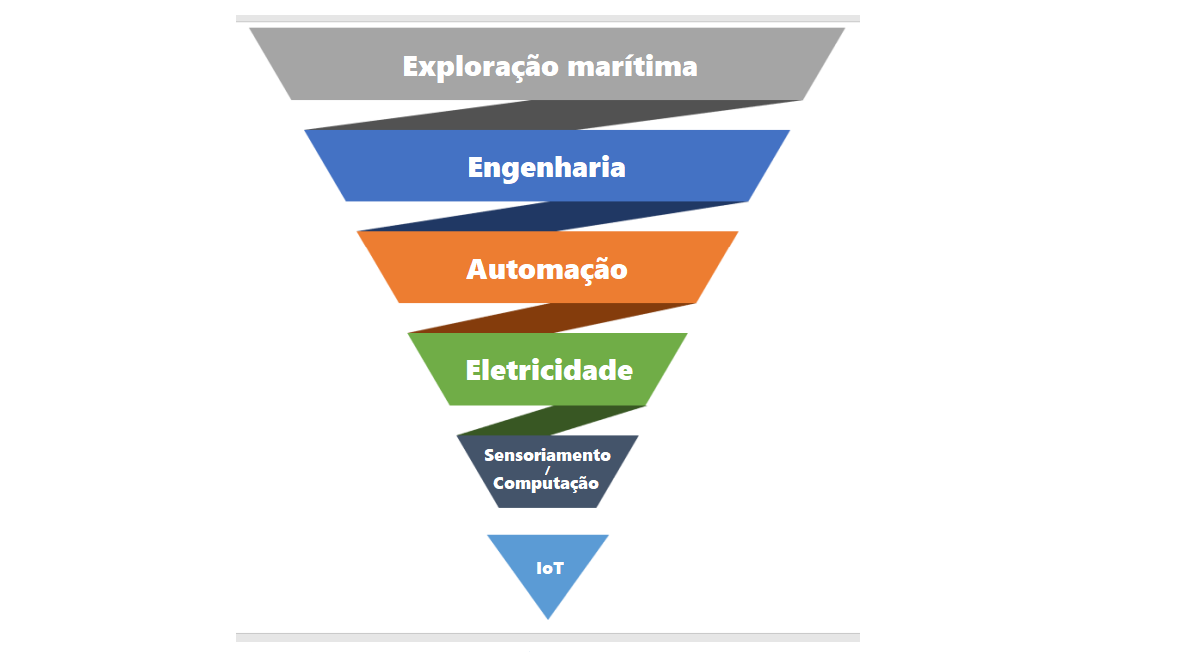
\includegraphics[width=10cm]{figuras/Datta.png}
    \fonte{Adaptado de \textcite{datta2017}.}
  \end{varwidth}
\end{figure}

\section{Protocolo HTTP}
De acordo com \textcite{RFC2616}, o Protocolo de Transferência de Hipertexto (HTTP) é um protocolo de comunicação utilizado para sistemas de informação distribuídos e colaborativos. Ele foi concebido para possibilitar a comunicação entre clientes e servidores na World Wide Web (WWW).

A concepção do HTTP remonta a 1989, quando Tim Berners-Lee propôs sua criação enquanto trabalhava no CERN, o Laboratório Europeu de Física de Partículas. A necessidade premente de compartilhar e distribuir informações de forma eficiente em uma rede de computadores motivou o desenvolvimento desse protocolo, que se tornou fundamental para a web moderna \parencite{Berners_web}. Ele é definido como:

\begin{quote}
"Um protocolo de camada de aplicação que define a estrutura de mensagens trocadas entre clientes e servidores. Ele opera sobre o Protocolo de Controle de Transmissão/Protocolo de Internet (TCP/IP), permitindo, nesta instância, a solicitação e transferência de recursos, como documentos HTML, imagens e vídeos, pela web." \parencite{RFC2616}
\end{quote}

No âmbito do desenvolvimento de sistemas, o HTTP desempenha um papel importante na criação de Interfaces de Programação de Aplicativos (APIs), possibilitando a comunicação entre diferentes componentes. Os desenvolvedores têm a capacidade de criar pontos de acesso HTTP (\textit{endpoints}) que aceitam solicitações e respondem com dados formatados, como JSON ou XML \parencite{Newmann_web}.

Na Tabela \ref{tab:metodos_http}, são destacados os principais métodos de solicitação do HTTP, utilizados para a interação entre clientes e servidores.

\begin{table}[!htb]
  \caption{Métodos HTTP} \label{tab:metodos_http}
  \begin{tabularx}{\textwidth}{|c|X|} \hline
    \textbf{Método} & \textbf{Descrição} \\ \hline
    GET & Solicita a representação de um recurso específico \\ \hline
    POST & Envia dados para serem processados por um recurso identificado no servidor \\ \hline
    PUT & Substitui todas as representações atuais do recurso de destino com os dados enviados na solicitação \\ \hline
    DELETE & Remove o recurso identificado no URI \\ \hline
    PATCH & Aplica modificações parciais a um recurso \\ \hline  
  \end{tabularx}
  \fonte{Adaptado de \textcite{RFC2616}.}
\end{table}

\section{Protocolo MQTT}

O MQTT (Message Queuing Telemetry Transport) foi introduzido pela primeira vez em 1999 por Dr. Andy Stanford-Clark, da IBM, e Arlen Nipper, da Arcom (agora Eurotech). Segundo \textcite{Andy_mqtt2004}, o MQTT foi inicialmente desenvolvido para o monitoramento de oleodutos e gasodutos através de comunicações de telemetria. Ele é definido como:

\begin{quote}
"Um método de transporte de dados leve para publicação e assinatura sobre TCP/IP com várias garantias de entrega. Otimizado para uso mínimo de largura de banda de rede e facilidade de implementação em sistemas embarcados, ele serve como um mecanismo de transporte onde é possível decidir o que enviar e quais ações tomar ao receber os dados." \parencite{Andy_mqtt2004}
\end{quote}

Nos sistemas embarcados, o MQTT é implementado nos dispositivos para permitir a troca de dados \parencite{Andy_mqtt2004}. Os dispositivos podem publicar dados de sensores e status usando tópicos MQTT, enquanto as aplicações podem se inscrever nesses tópicos para receber e processar os dados em tempo real \parencite{Yassein_mqtt2017}.

Do lado do servidor, os \textit{brokers} MQTT são implantados para gerenciar a troca de mensagens entre os dispositivos e as aplicações. Segundo \textcite{Yassein_mqtt2017}, esses \textit{brokers} são responsáveis por rotear as mensagens entre os clientes MQTT, garantindo a entrega dos dados. Além disso, os desenvolvedores podem usar bibliotecas MQTT em suas aplicações para se conectar aos \textit{brokers}, facilitando a implementação de funcionalidades de comunicação em seus sistemas \parencite{MQTT_org}.

Em sistemas IoT, o MQTT é utilizado para conectar dispositivos a plataformas de nuvem, permitindo o monitoramento e controle remoto dos dispositivos \parencite{junior2022data}. As aplicações podem processar os dados recebidos dos dispositivos IoT, realizar análises em tempo real e realizar ações com base nos eventos detectados \parencite{ferrandez2018precision,hsu2020creative}. Suas principais características são definidas na Tabela \ref{tab:caract_mqtt}.

\begin{table}[!htb]
  \caption{Características do protocolo MQTT} \label{tab:caract_mqtt}
  \begin{tabularx}{\textwidth}{|c|X|} \hline
    \textbf{Característica} & \textbf{Descrição} \\ \hline
    Leve & É leve e eficiente em termos de largura de banda e recursos de hardware \\ \hline
    Assíncrono & Dispositivos podem enviar e receber mensagens de forma independente, sem bloqueio ou espera ativa \\ \hline
    Padrão aberto & É um protocolo aberto e bem documentado \\ \hline
    Qualidade de Serviço (QoS) & Oferece três níveis de QoS para garantir a entrega confiável das mensagens: QoS 0 (entrega no máximo uma vez), QoS 1 (entrega pelo menos uma vez) e QoS 2 (entrega exatamente uma vez) \\ \hline
    Tópicos & Usa um modelo de publicação/assinatura, onde os dispositivos podem publicar mensagens em tópicos específicos e se inscrever para receber mensagens de tópicos de interesse \\ \hline  
    Baixa latência &  É projetado para minimizar a latência de rede, tornando-o adequado para casos de uso em tempo real, como telemetria, monitoramento e controle remoto \\ \hline
    Segurança & Suporta autenticação e criptografia \\ \hline
    Retenção de mensagens & Permite que o broker MQTT retenha as últimas mensagens publicadas em um tópico \\ \hline  
  \end{tabularx}
  \fonte{Adaptado de \textcite{MQTT_org}.}
\end{table}


\section{Gestão da irrigação}

A gestão eficaz da irrigação em regiões de escassez de água é um desafio que demanda pesquisa inovadora e sustentável, juntamente com a transferência apropriada de tecnologias \parencite{Burton_irrigation2010}. Considerando a complexidade das demandas e ofertas de recursos hídricos em perímetros irrigados, a utilização de técnicas e instrumentos é essencial para auxiliar profissionais nesse processo \parencite{Ramos_irrigacao2022}. Neste contexto, o conhecimento da variabilidade espacial dos atributos do solo relacionadas ao fluxo e armazenamento de água pode contribuir significativamente para a gestão eficiente da irrigação \parencite{Ramos_irrigacao2022}.

\textcite{Pereira_irrigation2002} discutem diversos aspectos relacionados à gestão da irrigação em propriedades agrícolas, incluindo o uso de águas residuais tratadas e águas salinas. Os autores destacam a importância de estratégias como a uniformidade de distribuição (DU) e práticas de irrigação suplementar (SI) e deficitária para reduzir a necessidade de água na agricultura \parencite{Pereira_irrigation2002, Ramos_irrigacao2022}.

Além disso, é ressaltada a necessidade de adotar tecnologias emergentes para o gerenciamento de água e desenvolver metodologias para analisar os benefícios sociais, econômicos e ambientais da melhoria da gestão da irrigação, como destacado por \textcite{Burton_irrigation2010}.

Essa integração de técnicas, ferramentas computacionais e modelos de distribuição espacial dos atributos do solo, aliada à espacialização dos dados, proporciona uma abordagem mais eficiente para a gestão da irrigação em áreas específicas, melhorando assim o uso da água em escalas como a de um perímetro irrigado \parencite{Burton_irrigation2010, Ramos_irrigacao2022}.

\section{Gestão baseada no consumo de água}

Segundo \textcite{carmody_fao2023}, a gestão baseada no consumo de água (CBWM) traz uma perspectiva inovadora ao considerar não apenas a entrega de água, mas o uso real da mesma na agricultura, o que contribui para a eficiência do uso dos recursos hídricos e para a sustentabilidade dos sistemas agrícolas. A CBWM reconhece que a água pode ser consumida de forma benéfica, como na transpiração das plantas para a produção de alimentos, ou de forma não benéfica, como na evaporação do solo nu ou superfícies de água nuas. Além disso, destaca a importância dos fluxos de retorno não consumidos, que podem ser recuperados para consumo benéfico ou manter os ecossistemas aquáticos (Figura \ref{figura:ciclo_agua}), contribuindo para o abastecimento de outros usuários a jusante e para a saúde dos rios e lençóis freáticos \parencite{carmody_fao2023}.

\textcite{carmody_fao2023} ainda complementa que para alcançar economias reais de água, é necessário atender a quatro requisitos no contexto de um quadro mais amplo, onde os fluxos ambientais são considerados para sustentar esses sistemas e as pessoas que dependem deles. Esses requisitos incluem a determinação dos requisitos específicos de evapotranspiração (ET) para a produção de culturas, a definição dos direitos de água em termos de extração, consumo e fluxos de retorno, o uso do monitoramento de ET e cobertura do solo para ajustar as alocações de água, e a comparação da ET alvo com a ET real para garantir um balanço hídrico adequado \parencite{Allen_evapotranspiration1998, carmody_fao2023}.

A gestão eficaz da irrigação não apenas envolve a aplicação de técnicas e tecnologias específicas, mas também requer uma compreensão abrangente dos princípios subjacentes ao uso sustentável da água na agricultura, como os propostos pela CBWM \parencite{Ramos_irrigacao2022, carmody_fao2023}.

\begin{figure}[!htb] \centering
  \caption{Ciclo Hidrológico} \label{figura:ciclo_agua}
  \begin{varwidth}{\linewidth}
    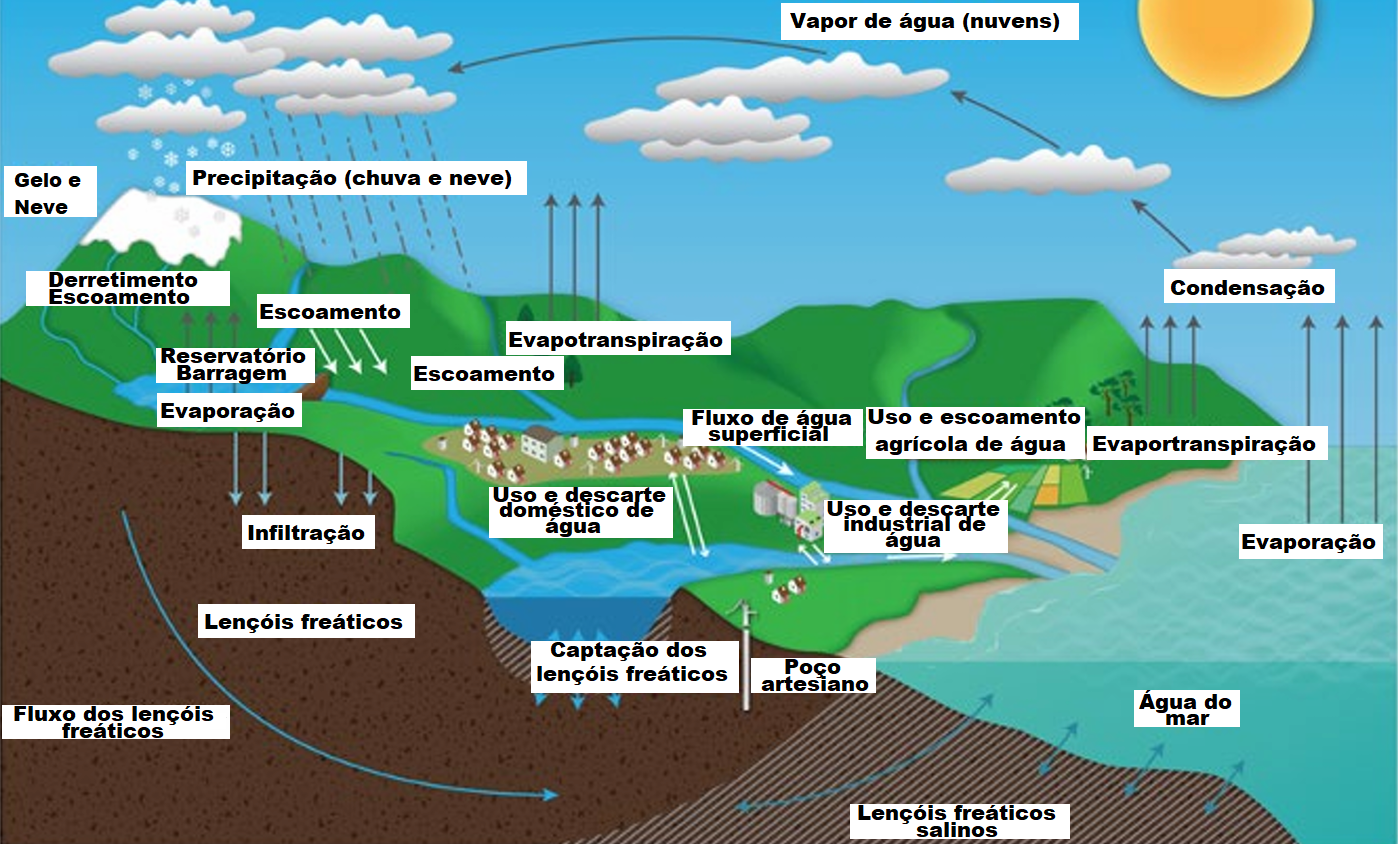
\includegraphics[width=16cm]{figuras/Carmody.png}
    \fonte{Adaptado de \textcite{carmody_fao2023}.}
  \end{varwidth}
\end{figure}

\section{Evapotranspiração}

A evapotranspiração (ET) descreve o processo fundamental de transferência de água da superfície da Terra para a atmosfera \parencite{carmody_fao2023}. Como ilustrado no ciclo hidrológico (Figura \ref{figura:ciclo_agua}), a ET desempenha um papel essencial na dinâmica hídrica. Foi observado que:

\begin{quote}
  "Três tipos de superfície são importantes no retorno da chuva à atmosfera. Para extensas áreas de terra, são eles, em ordem de importância: vegetação, na qual as folhas das plantas atuam como superfícies transpirantes; solo nu ou pousio, de onde a água evapora na interface solo-ar ou logo abaixo dela e em águas abertas, a partir das quais a evaporação ocorre diretamente." \parencite{Penman_evapotranspiration1948}
\end{quote}

\textcite{Penman_evapotranspiration1948} ainda complementa que a irrigação, ao fornecer água ao solo, influencia diretamente a evaporação subsequente, afetando não apenas a quantidade de água disponível para evaporação, mas também a temperatura e a umidade do solo, que por sua vez impactam a taxa de evaporação.

O aumento da ET global é um fenômeno de grande relevância no contexto atual das mudanças climáticas. Como mencionado por \textcite{yang_nature2023}, observa-se uma tendência multi-decadal de aceleração no aumento da ET desde a década de 1980. Essas mudanças são fortemente relacionadas ao crescimento da vegetação e da área plantada, evidenciado pelo aumento do índice de área foliar (LAI).

A ET de referência (ETo) pode ser calculada utilizando o método recomendado pela FAO-56 \parencite{Allen_evapotranspiration1998}, definido pela equação:

\begin{equation}
ETo = 0.408 \cdot \frac{\Delta (R_n - G) + \gamma \cdot \frac{900}{T + 273} \cdot u2 \cdot (e_s - e_a)}{\Delta + \gamma \cdot (1 + 0.34 \cdot u2)}
\end{equation}

Onde:
\begin{itemize}
  \item $ETo$ é a evapotranspiração de referência (mm/dia)
  \item $R_n$ é a radiação líquida (MJ/m$^2$/dia)
  \item $G$ é o calor do solo (MJ/m$^2$/dia)
  \item $\Delta$ é o déficit de pressão de vapor (kPa/°C)
  \item $\gamma$ é a constante psicrométrica (kPa/°C)
  \item $T$ é a temperatura média do ar (°C)
  \item $u2$ é a velocidade do vento a 2 metros de altura (m/s)
  \item $e_s$ é a pressão de vapor do ar saturado (kPa)
  \item $e_a$ é a pressão de vapor do ar (kPa)
\end{itemize}

A ET de cultura (ETc) é calculada como o produto da ETo e um coeficiente de cultura ($Kc$) específico para cada cultura, como proposto por \textcite{bernardo_irrigacao2006}:

\begin{equation}
ETc = Kc \times ETo
\end{equation}

Métodos de telemetria da ETo têm mostrado resultados promissores na compreensão desse fenômeno em escalas regional e global. De acordo com as revisões feitas por \textcite{Zhang_evapotranspiration_med2016, Zhao_evapotranspiration_med2009}, esses métodos variam desde modelos de equações simplificadas até modelos de balanço energético de duas fontes mais complexos. Eles frequentemente utilizam dados multiespectrais remotamente detectados, abrangendo desde o visível até as bandas infravermelhas térmicas. 

No entanto, muitos desses modelos dependem, em certa medida, de medições auxiliares baseadas em solo para derivar os fluxos de calor turbulentos em uma escala regional \parencite{Zhao_evapotranspiration_med2009, Zhang_evapotranspiration_med2016}.

O método com melhores resultados para medição de ETo é apresentado por \textcite{Yang_evapotranspiration_med2022}, em que é realizada a fusão de dados de diferentes satélites (Landsat 8 e o Sentinel-2) com resoluções espaciais e temporais variáveis, o que proporciona uma estimativa mais contínua da ET diária em escala de campo.